\chapter*{Mathe-Challenge}

\section*{Arithmetik}

i). Berechnen Sie den Wert des Produkts von Brüchen $$\left(\frac{60}{21}\right)\times\left(\frac{1}{33}\right)\times\left(\frac{6}{5}\right)\times \left(\frac{35}{8}\right)$$\\

%Sug: 1. ¿Cómo se multiplican las fracciones?. 2. Factoriza y cancela (no se tiene que hacer ninguna multiplicación). Recuerda que el orden de los factores no altera el producto (tanto el de arriba como el de abajo). \\

ii). Finden Sie den Produkt. $$\left(\frac{1}{2}\right)\times\left(\frac{2}{3}\right)\times\left(\frac{3}{4}\right)\times\cdots \times\left(\frac{998}{999}\right)\times\left( \frac{999}{1000}\right).$$

iii). Berechnen Sie die Summe der ersten dreiunddreißig natürlichen Zahlen $$1+2+3+4+5+\cdots+31+32 +33?$$

iv). Bestimmen Sie die Summe $$1+2+3+4+\cdots +1998+1999+2000.$$

%Sug: El problema v) es más sencillo. Inténtalo primero. 1A. Suma dos veces (al derecho y al revés). 1B. Arreglo triangular de puntos. \\

v). Berechnen Sie die Summe der ersten tausend ungeraden Zahlen: $$1+3+5+7+\cdots +1995+1997+1999.$$

%Sug: A. Arreglo cuadrangular de puntos, o B. Suma dos veces (al derecho y al revés). \\

vi). Bestimmen Sie die Summe $$1+2+2^2+2^3+\cdots +2^{18}+2^{19}.$$

%Sug: 1. Haz una conjetura directa revisando casos pequeños: 1, 1+2, 1+2+4, 1+2+4+8, \dots 2. ¿Cómo se ven esos números en base binaria?. \\

vii). Diesmal mit Potenzen von drei: $$1+3+3^2+3^3+\cdots +3^{18}+3^{19}$$

%Sug: 1. Usa base tres. 2. Multiplica por dos y suma uno. \\

viii). Versuchen Sie, die Summe von Kubikzahlen zu bestimmen: $$1^3+2^3+3^3+4^3+\cdots +98^3+99^3+100^3$$

%Sug: Haz una conjetura directa revisando casos pequeños. \\

ix). Jetzt versuchen Sie mit Quadratzahlen: $$1^2+2^2+3^2+4^2+\cdots +98^2+99^2+100^2.$$

%Sug: Aquí no es nada fácil obtener una conjetura directa (cough!, cough!, $\frac{1}{6}n(n+1)(2n+1)$).\\

x). Bestimmen Sie den Wert von $$1\times2+2\times3+3\times4+\cdots +99\times100+100\times101.$$

%Sug: Suma los ejercicios v) y ix).\\

%Notas al Instructor: i) y ii). Revisar manejo de operaciones de fracciones. iii)-v). Preguntar cómo llegaron al resultado. No anticipar truco de sumar dos veces al derecho y al revés. vi) y vii). Revisar manejo de bases numéricas.  viii)-x). Invitación a la inducción matemática: ¿Cuánto vale la diferencia de términos consecutivos de tu fórmula?. Repaso de manejo de sumas y multiplicaciones de fracciones con variables. \\

\vspace{1cm}
(Fragen/Hinweise/Lösungen: ei.turbomath@gmail.com)

\newpage

\section*{Schachbretter und Tetris-Blöcke}

\begin{multicols}{2}
i). Sie bekommen zehn Tetris-Blöcke, zwei von jedem Typ (Abb. 1). Entscheiden Sie:

Ist es möglich, mit den zehn Blöcken, ein Rechteck (ohne Löcher) zusammenzufügen? Die Blöcken dürfen nicht übereinander stehen!.\\

%Sug: Intenta con un rectángulo de 8\times 5. \\

ii). Wenn jetzt drei Blöcke von jedem Typ benutzen werden müssen: Ist es möglich oder nicht?\\

%Sug: Mejor piénsale primero al iii) y al iv). \\

iii). Zwei gegenüberliegende Ecken eines Schachbrettes werden entfernt (s. Abb. 2).  

Ist es möglich, den Rest mit genau dreiunddreißig $(2\times 1)$ Domino-Fliesen zu bedecken?\\

%Sug: ¿De qué colores son las esquinas? Intenta primero con tableros más pequeños. \\

iv). Betrachten Sie ein $(5\times 5)$-Schachbrett mit drei
Ecken entfernt, wie in Abbildung 3.
  
Ist es möglich, den Rest des Schachbrettes mit elf Domino-Fliesen zu bedecken??\\

%Sug: ¿De qué colores son las esquinas?

v). Es ist möglich, ein $(7\times 7)$-Schachbrett mit sechzehn $(3\times 1)$-Blöcke und einem einzelnen $(1\times 1)$-Block zu bedecken.

Markieren Sie alle möglichen Orte der $(1\times 1)$-Block (Abbildung 4).

%Sug: No se pueden todas. Colorear con tres colores por diagonales para descartar algunas posiciones.

\columnbreak

\begin{tikzpicture}[line cap=round,line join=round,>=triangle 45,x=.5cm,y=.5cm]
\draw [line width=1pt] (0,0)-- (2,0);
\draw [line width=1pt] (0,0)-- (0,2);
\draw [line width=1pt] (0,2)-- (2,2);
\draw [line width=1pt] (2,2)-- (2,0);
\draw [line width=1pt] (0,1)-- (2,1);
\draw [line width=1pt] (1,2)-- (1,0);
\draw [line width=1pt] (5.6,2.6)-- (7.6,2.6);
\draw [line width=1pt] (7.6,2.6)-- (7.6,0.6);
\draw [line width=1pt] (6.6,0.6)-- (8.6,0.6);
\draw [line width=1pt] (8.6,0.6)-- (8.6,1.6);
\draw [line width=1pt] (8.6,1.6)-- (5.6,1.6);
\draw [line width=1pt] (5.6,2.6)-- (5.6,1.6);
\draw [line width=1pt] (6.6,2.6)-- (6.6,0.6);
\draw [line width=1pt] (0,4)-- (0,7);
\draw [line width=1pt] (0,7)-- (1,7);
\draw [line width=1pt] (1,7)-- (1,4);
\draw [line width=1pt] (1,4)-- (0,4);
\draw [line width=1pt] (0,5)-- (1,5);
\draw [line width=1pt] (1,6)-- (0,6);
\draw [line width=1pt] (4.5,1.2)-- (4.5,4.2);
\draw [line width=1pt] (3.5,4.2)-- (3.5,1.2);
\draw [line width=1pt] (2.5,3.2)-- (4.5,3.2);
\draw [line width=1pt] (2.5,2.2)-- (4.5,2.2);
\draw [line width=1pt] (2.5,3.2)-- (2.5,2.2);
\draw [line width=1pt] (3.5,4.2)-- (4.5,4.2);
\draw [line width=1pt] (3.5,1.2)-- (4.5,1.2);
\draw [line width=1pt] (2,7)-- (2,5);
\draw [line width=1pt] (3,5)-- (3,7);
\draw [line width=1pt] (2,7)-- (5,7);
\draw [line width=1pt] (5,6)-- (2,6);
\draw [line width=1pt] (2,5)-- (3,5);
\draw [line width=1pt] (4,7)-- (4,6);
\draw [line width=1pt] (5,7)-- (5,6);
\draw [line width=1pt] (0,4)-- (0,3);
\draw [line width=1pt] (0,3)-- (1,3);
\draw [line width=1pt] (1,3)-- (1,4);
\end{tikzpicture}

Fig. 1: Fünf Art

Tetris-Blöcke <<gerade>>, <<L>>,  

<<Quadrat>>, <<T>> y <<Z>> \\

    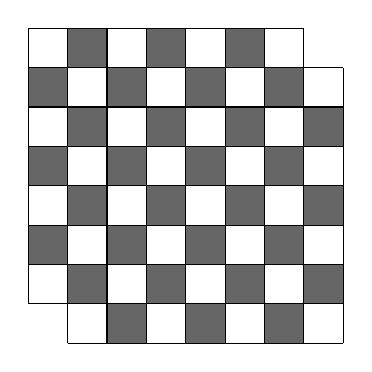
\begin{tikzpicture}[x=0.5cm,y=0.5cm]
  \foreach \i in {0,...,3} 
    \foreach \j in {0,...,3}
    \fill[line width=1pt,color=black,fill=black,fill opacity=0.6] (2*\i,2*\j) -- (2*\i,2*\j+1) -- (2*\i+1,2*\j+1) -- (2*\i+1,2*\j) -- cycle;
  \foreach \i in {0,...,3} 
    \foreach \j in {0,...,3}
        \fill[line width=1pt,color=black,fill=black,fill opacity=0.6] (2*\i+1,2*\j+1) -- (2*\i+1,2*\j+2) -- (2*\i+2,2*\j+2) -- (2*\i+2,2*\j+1) -- cycle;
        \fill[line width=1pt,color=white,fill=white,fill opacity=1] (0,0) -- (0,1) -- (1,1) -- (1,0) -- cycle;
        \fill[line width=1pt,color=white,fill=white,fill opacity=1] (7,7) -- (7,8) -- (8,8) -- (8,7) -- cycle;
    \foreach \i in {1,...,7} \draw[black] (0,\i) -- (8,\i);
    \foreach \i in {1,...,7} \draw[black] (\i,0) -- (\i,8);       
    \draw[black] (1,0) -- (8,0);
    \draw[black] (0,1) -- (0,8);
    \draw[black] (0,8) -- (7,8);
    \draw[black] (8,0) -- (8,7);
  \end{tikzpicture}

Fig. 2

 \end{multicols}
    
 Fig. 3 \hspace{.5cm}
  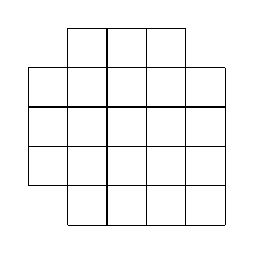
\begin{tikzpicture}[x=0.5cm,y=0.5cm]
     \foreach \i in {1,...,4} \draw[black] (0,\i) -- (5,\i);
    \foreach \i in {1,...,4} \draw[black] (\i,0) -- (\i,5);       
    \draw[black] (1,0) -- (5,0);
    \draw[black] (0,1) -- (0,4);
    \draw[black] (1,5) -- (4,5);
    \draw[black] (5,0) -- (5,4);
  \end{tikzpicture}
  \hspace{3cm} Fig. 4 \hspace{.5cm}  
  
\begin{tikzpicture}[x=0.5cm,y=0.5cm]
     \foreach \i in {0,...,7} \draw[black] (0,\i) -- (7,\i);
    \foreach \i in {0,...,7} \draw[black] (\i,0) -- (\i,7);       
  \end{tikzpicture}
  \\
   
  vi). Betrachten Sie ein $(2n)\times(2n)$-Schachbrett, ohne seine vier Ecken, wie in Abb. 5.

Sie dürfen nur L-förmige Tetris-Blöcke verwenden. Für welche Werte $n=1,2,3,4,5,\dots$ ist es möglich, den Rest des Bretts abzudecken?

%Sug: i) Algunos se pueden y algunos no se pueden. ii) Para descartar n=2k, colorear con franjas negras y blancas. iii) ¿Es posible cubrir $n=b$ casillas con un número impar de tetraminos <<L>>?
Fig. 5\hspace{.5cm}
  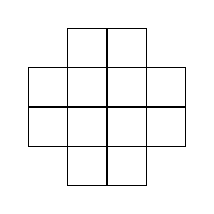
\begin{tikzpicture}[x=0.5cm,y=0.5cm]
     \foreach \i in {1,...,3} \draw[black] (0,\i) -- (4,\i);
    \foreach \i in {1,...,3} \draw[black] (\i,0) -- (\i,4);       
    \draw[black] (1,0) -- (3,0);
    \draw[black] (0,1) -- (0,3);
    \draw[black] (1,4) -- (3,4);
    \draw[black] (4,1) -- (4,3);
  \end{tikzpicture}
  $n=2$
  \hspace{.5cm}  
    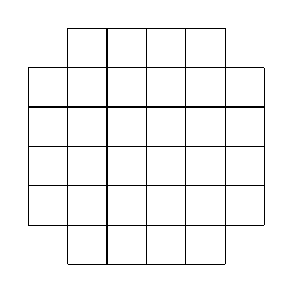
\begin{tikzpicture}[x=0.5cm,y=0.5cm]
     \foreach \i in {1,...,5} \draw[black] (0,\i) -- (6,\i);
    \foreach \i in {1,...,5} \draw[black] (\i,0) -- (\i,6);       
    \draw[black] (1,0) -- (5,0);
    \draw[black] (0,1) -- (0,5);
    \draw[black] (1,6) -- (5,6);
    \draw[black] (6,1) -- (6,5);
  \end{tikzpicture}
  $n=3$
   \hspace{.5cm}
   
\begin{tikzpicture}[x=0.5cm,y=0.5cm]
     \foreach \i in {1,...,7} \draw[black] (0,\i) -- (8,\i);
    \foreach \i in {1,...,7} \draw[black] (\i,0) -- (\i,8);       
    \draw[black] (1,0) -- (7,0);
    \draw[black] (0,1) -- (0,7);
    \draw[black] (1,8) -- (7,8);
    \draw[black] (8,1) -- (8,7);
  \end{tikzpicture}
  $n=4$. 

%Notas al Instructor: i) Ejercicio tipo <<puzzle>>. ii)-iv) Ejemplos de problemas que se justifican con el <<Principio de invarianza>>. En iii) y iv), los más sencillo, siempre hay $n=2+b$ casillas negras y $b$ blancas, pues cada dominó (en cualquier posición) cubre una negra y una blanca. En ii) una cantidad impar de tetraminos <<T>> impiden la construcción (pues no se puede cubrir $n=b$ con un número impar de <<T>>'s). v) Dos posibles coloraciones por diagonales a tres colores. Abreviar casos posibles usando simetrías / modificaciones locales. vi) se requiere un argumento de coloración (por franjas) y un argumento de paridad. 
 
\begin{multicols}{2}
\section*{Geometrie: Flächen}

i). Betrachten Sie ein Dreieck $ABC$ mit Seiten $|AB|=3$ und $|BC|=4$. Der Winkel $\measuredangle BAC=30^{\circ}$, wie in Abbildung 1. Bestimmen Sie die Fläche des Dreiecks (Hinweis: $\sin(30^{\circ})=\frac{1}{2}$).

%Sug: La altura del triángulo es $h=b\cdot \sen(30^{\circ})$. De hecho, en general, el área de un triángulo es $\frac{1}{2}\cdot b\cdot c \cdot \sen(\apha)$

ii). Auf dem Einheitskreis ist ein regulär Zwölfeck eingeschrieben, wie in Abbildung 2. Berechnen Sie die Fläche des Zwölfecks.\\
%Sug: ¿Cuál es el área de cada uno de los doce sectores triangulares?.

iii). Berechnen Sie die Fläche eines regelmäßigen $360$-Ecks, das im Einheitskreis einbeschrieben ist. (Hinweis: $\sin(1^{\circ})=0,0174524\dots$)\\
%Sug: ¿Cuál es el área de cada uno de los $360$ sectores triangulares?.

iv). Berechnen Sie die Fläche der Muschel aus Abbildung 3, wobei:\\

Die Winkel zwischen aufeinanderfolgenden Strahlen vom Zentrum sind alle gleich $30^{\circ}$.\\

Die Längen der 13 Strahlen sind arithmetisch fortschreitend: \\

$l_1=1, l_2=2, l_3=3, l_4=4, \dots, l_{13}=13$. 

%Sug: Te puede ayudar la fórmula para el ejercicio x) de aritmética.

\section*{Teiler und Reste}

Ein Teiler einer ganzen Zahl $n$ ist eine andere ganze Zahl $d$, sodass der Bruch $\frac{n}{d}=q$ wieder eine ganze Zahl ist, $n=d\times q$. 

Zum Beispiel: die Zahl $n=6$ besitzt vier positive Teiler: $d=1,2,3,6$ ($\frac{6}{1}=6$, $\frac{6}{2} =3$, $\frac{6}{3}=2$, $\frac{6}{6}=1$ sind ganze Zahlen, aber $\frac{6}{4}=1,5$ y $ \frac{6}{5}=1,2$ nicht).

\columnbreak

\definecolor{qqwuqq}{rgb}{0,0.39215686274509803,0}
\definecolor{qqqqff}{rgb}{0,0,1}
\definecolor{ududff}{rgb}{0.30196078431372547,0.30196078431372547,1}
\begin{tikzpicture}[line cap=round,line join=round,>=triangle 45,x=1.5cm,y=1.5cm]
\draw [shift={(0,0)},line width=1pt,color=black,fill=black,fill opacity=0.10000000149011612] (0,0) -- (0:0.2580645161290323) arc (0:30:0.2580645161290323) -- cycle;
\draw [line width=1pt] (0,0)-- (2.598076211353316,1.5);
\draw [line width=1pt] (0,0)-- (4,0);
\draw [line width=1pt] (2.598076211353316,1.5)-- (4,0);
\draw[color=black] (-0.2313802083333099,0.22449680779561737) node {$A$};
\draw[color=black] (4.190125168010777,0.03524949596765889) node {$C$};
\draw[color=black] (2.5299101142473357,1.7986903561827265) node {$B$};
\draw[color=black] (1.3944262432795937,1.1) node {$c=3$};
\draw[color=black] (2.03098538306454,-0.2) node {$b=4$};
\draw[color=black] (0.85,0.2) node {$\alpha = 30^{\circ}$};
\end{tikzpicture}

Fig.1

\definecolor{uuuuuu}{rgb}{0.26666666666666666,0.26666666666666666,0.26666666666666666}
\definecolor{xdxdff}{rgb}{0.49019607843137253,0.49019607843137253,1}
\definecolor{ududff}{rgb}{0.30196078431372547,0.30196078431372547,1}
\begin{tikzpicture}[line cap=round,line join=round,>=triangle 45,x=2.5cm,y=2.5cm]
\draw [line width=1pt] (0,0)-- (1,0);
\draw[color=black] (0.3,0.1) node {$r=1$};
\draw [line width=1pt] (1,0)-- (0.8660254037844387,0.5);
\draw [line width=1pt] (0.8660254037844387,0.5)-- (0.5,0.8660254037844386);
\draw [line width=1pt] (0.5,0.8660254037844386)-- (0,1);
\draw [line width=1pt] (0,1)-- (-0.5,0.8660254037844386);
\draw [line width=1pt] (-0.5,0.8660254037844386)-- (-0.8660254037844383,0.5);
\draw [line width=1pt] (-0.8660254037844383,0.5)-- (-1,0);
\draw [line width=1pt] (-1,0)-- (-0.8660254037844386,-0.5);
\draw [line width=1pt] (-0.8660254037844386,-0.5)-- (-0.5,-0.8660254037844384);
\draw [line width=1pt] (-0.5,-0.8660254037844384)-- (0,-1);
\draw [line width=1pt] (0,-1)-- (0.5,-0.8660254037844388);
\draw [line width=1pt] (0.5,-0.8660254037844388)-- (0.8660254037844384,-0.5);
\draw [line width=1pt] (0.8660254037844384,-0.5)-- (1,0);
\end{tikzpicture}

Fig. 2

\begin{tikzpicture}[line cap=round,line join=round,>=triangle 45,x=.3cm,y=.3cm]
\draw [line width=1pt] (0,0)-- (1,0);
\draw [line width=1pt] (1,0)-- (1.7320508075688774,1);
\draw [line width=1pt] (1.7320508075688774,1)-- (1.5,2.598076211353316);
\draw [line width=1pt] (1.5,2.598076211353316)-- (0,4);
\draw [line width=1pt] (0,4)-- (-2.5,4.3301270189221945);
\draw [line width=1pt] (-2.5,4.3301270189221945)-- (-5.196152422706631,3);
\draw [line width=1pt] (-5.196152422706631,3)-- (-7,0);
\draw [line width=1pt] (-7,0)-- (-6.928203230275514,-4);
\draw [line width=1pt] (-6.928203230275514,-4)-- (-4.5,-7.794228634059941);
\draw [line width=1pt] (-4.5,-7.794228634059941)-- (0,-10);
\draw [line width=1pt] (0,-10)-- (5.5,-9.526279441628834);
\draw [line width=1pt] (5.5,-9.526279441628834)-- (10.392304845413255,-6);
\draw [line width=1pt] (10.392304845413255,-6)-- (13,0);
\draw [line width=1pt] (0,0)-- (1.7320508075688774,1);
\draw [line width=1pt] (0,0)-- (1.5,2.598076211353316);
\draw [line width=1pt] (0,0)-- (0,4);
\draw [line width=1pt] (0,0)-- (-2.5,4.3301270189221945);
\draw [line width=1pt] (0,0)-- (-5.196152422706631,3);
\draw [line width=1pt] (0,0)-- (-7,0);
\draw [line width=1pt] (0,0)-- (-6.928203230275514,-4);
\draw [line width=1pt] (0,0)-- (-4.5,-7.794228634059941);
\draw [line width=1pt] (0,0)-- (0,-10);
\draw [line width=1pt] (0,0)-- (5.5,-9.526279441628834);
\draw [line width=1pt] (0,0)-- (10.392304845413255,-6);
\draw [line width=1pt] (1,0)-- (13,0);
\draw[color=black] (-4.3475,-4.305) node {$\ddots$};
\draw[color=black] (-1.7575,-6.06) node {$l_{9}=9$};
\draw[color=black] (0.375,-7.635) node {$l_{10}=10$};
\draw[color=black] (5.4875,-5.475) node {$l_{11}=11$};
\draw[color=black] (6.7625,-2.325) node {$l_{12}=12$};
\draw[color=black] (7.3975,0.69) node {$l_{13}=13$};
\end{tikzpicture}

Fig. 3

\end{multicols}

Die Zahl $n=18$ besitzt sechs positive Teiler: $d=1,2,3,6,9,18$. Die Zahl $d=7$ ist kein Teiler von $18$, da $\frac{18}{7}=2+\frac{4}{7}$ keine ganze Zahl ist. Der Quotient ist $2$ und der Rest ist $4$.\\

i). Wie viele positive Teiler besitzt $n=360$?\\

ii). Wie viele positive Teiler besitzt $n=10008000$?\\

%Sug: Si n=p_1^{\alpha_1}p_2^{\alpha_2}p_3^{\alpha_3}\cdots p_k^{\alpha_k}. Entonces $n$ tiene exactamente $(\alpha_+1)(\alpha_2+1)(\alpha_3+1)\dots (\alpha_k+1) divisores. ¿Por qué?.

iii). Was ist der Rest von $n=100080001$, dividiert durch neun?\\

%Sug: 1+8+1. ¿Por qué? 

iv). Was ist der Rest von $n=2021^{2021}+2020^{2020}$ dividiert durch neun?\\

%Sug: Observar cómo se comportan los residuos entre nueve de $2020^1, 2020^2, 2020^3, 2020^4, 2020^5, \dots$. Comparar con $4^1, 4^2, 4^3, 4^4, 4^5, \dots$.

v). Finden Sie die kleinste natürliche ganze Zahl $n$, so dass:
\begin{itemize}
\item der Rest von $n$, dividiert durch $7$, ist $6$,
\item der Rest von $n$, dividiert durch $11$, ist $10$,
\item der Rest von $n$, dividiert durch $13$, ist $12$,.
\end{itemize}

%Sug: $7\cdot 11 \cdot 13 =1001$.

\section*{Algebra}

Wir erinnern uns an die Expansion und Reduktion von Potenzen des Binoms $(x+y)^n$. Für $n=2,3$:
$$(x+y)^2=(x+y)(x+y)=xx+xy+yx+yy= x^2+2xy+y^2,$$
$$(x+y)^3=(x+y)(x+y)(x+y)=\dots = x^3+3x^2y+3xy^2+y^3.$$

i). Bestimmen Sie den Koeffizienten des Terms $x^3y^6$, nach der Vereinfachung des Ausdrucks $(x+y)^{9}$.\\

ii). Berechnen den Koeffizienten des Terms $x^2y^3z^4$, nach der Vereinfachung des Ausdrucks $(x+y+z)^{9}$.

%Sug: Triángulo de Pascal.

\section*{Stochastik}

i) Sie werfen eine faire Münze sieben Mal. Berechnen Sie die Wahrscheinlichkeit, <<Kopf>> genau viermal zu erhalten.\\

%Sug: El n-ésimo renglón triángulo de Pascal indica las probabilidades de obtener k=0,1,2,\dots n veces <<cara>>. ¿Por qué?. 

ii) Welches Ereignis ist wahrscheinlicher?:

a). Sechs Würfel zu werfen und mindestens einmal <<vier>> zu erhalten.

b). Zwölf Würfel zu werfen und mindestens zweimal <<sechs>> zu erhalten.\\

iii) Betrachten Sie das folgende Münzwurfspiel: Sie werfen achtmal eine Münze...

Wenn Sie eine gerade Anzahl von <<Köpfen>>  bekommen ($0,2,4,6$ oder $8$), verlieren Sie $1\$ $,

Wenn Sie eine ungerade Anzahl von <<Köpfen>> erhalten ($1,3,5$ oder $7$), verdienen Sie $(1,50)\$$,

Wie empfehlenswert ist, dieses Spiel zu spielen?\\

iv) Die Spielregeln <<Trez loko>> lauten wie folgt:

Eintritt kostet $1\$$. Man wirft zehn Würfeln und zählt, wie viele <<dreier>> erhalten sind.

Falls drei oder mehr: Sie verdienen $3\$$.

Soll ich mein Glück bei <<Trez loko>> versuchen? 

\section*{Trigonometrie}

Erinnern Sie sich an die trigonometrischen Identitäten für Winkelsummen:
$$\cos(\alpha+\beta)=\cos(\alpha)\cos(\beta)-\sin(\alpha)\sen(\beta), \quad \sin(\alpha+\beta)=\cos(\alpha)\sin(\beta)+\sin(\alpha)\cos(\beta)$$

i). Drücken Sie $\sin(3\alpha)$ und $\cos(3\alpha)$ durch $\sin(\alpha)$ und $\cos(\alpha)$ aus.\\

ii). Drücken Sie  $\sin(7\alpha)$ und $\cos(6\alpha)$ durch $\sin(\alpha)$ und $\cos(\alpha)$ aus.

%Sug: Triángulo de Pascal y números complejos (identidad de Euler).

\section*{Infinitesimalrechnung}

i). Berechnen Sie den Wert der folgenden Limes:

$$\lim_{n\to\infty}=\frac{n}{2}\sin\left(\frac{2 \pi}{n} \right).$$

%Sug: Problemas ii) y iii) de áreas.

ii). Warum ist die Ableitung der Funktion $f(x):=x^n$ gleich $f'(x)=nx^{n-1}$?\\

%Sug: Aplicar el teorema del binomio a $(x+h)^n$

iii). Warum sind die Ableitungen der Funktionen $f(x):=\cos(x)$ und $g(x):=\sin(x)$ gleich $$f'(x)=\sin(x), \quad g'(x)=-\cos(x)?$$
